%Assignment 2 
%Vikas Kurapati
%130010058
\documentclass[11pt, a4paper]{article}
\usepackage[affil-it]{authblk} 
\usepackage{etoolbox}
\usepackage{lmodern}
\usepackage{titlesec}
\usepackage{float}

\makeatletter
\patchcmd{\@maketitle}{\LARGE \@title}{\fontsize{20}{19.2}\selectfont\@title}{}{}
\makeatother

\renewcommand\Authfont{\fontsize{16}{14.4}\selectfont}
\renewcommand\Affilfont{\fontsize{12}{10.8}\itshape}

\title{\textbf{Assignment 4}} 
\author{Vikas Kurapati - 130010058}
\usepackage{graphicx}
\begin{document}
\maketitle
\newpage
\section{Question1:}
Refer code. \\
It takes of the order of 1.56721581558s to consider it as a steady state.

\section{Question 2}
Distribution function is given as
\begin{figure}[H]
 \centering
 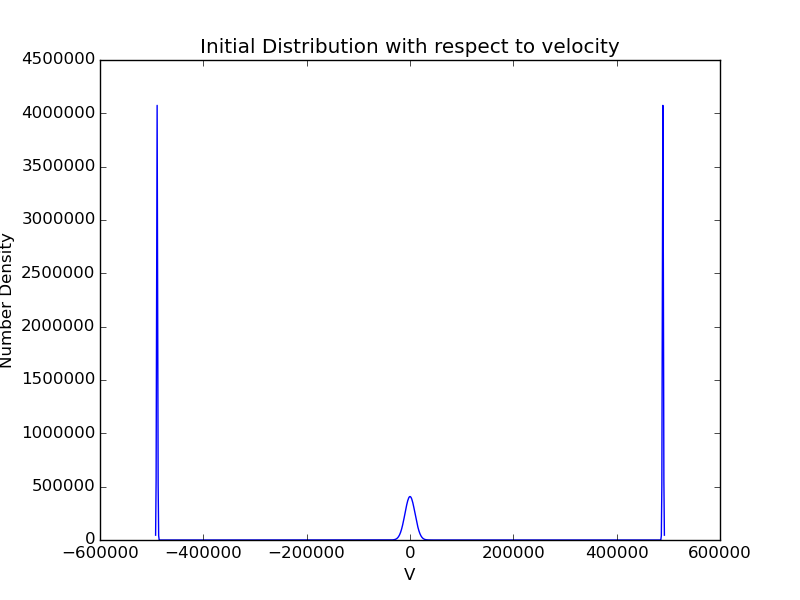
\includegraphics[width = \textwidth]{q2.png}
\end{figure}

\section{Question 3}
Refer code. \\
The density computed numerically is about 0.042854309082 and temperature is about 1.16683191751e+15eV

\section{Question 4}
The equilibrium distribution function is given by
\begin{figure}[H]
 \centering
 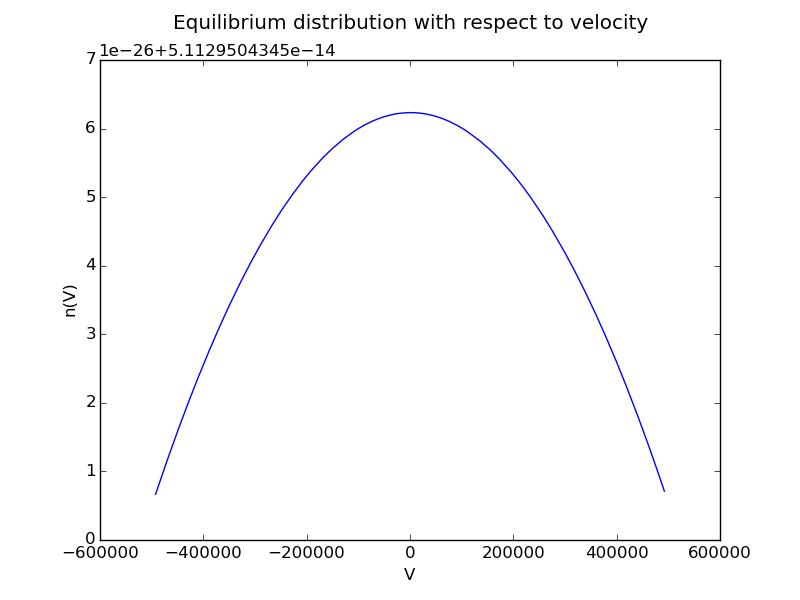
\includegraphics[width = \textwidth]{q4.png}
\end{figure}

\section{Question5}
Refer code. \\
It takes of the order of 65.9797858359 s to deviate from maxwellian.

\section{Question6}
The development of entropy is given as follows.
\begin{figure}[H]
 \centering
 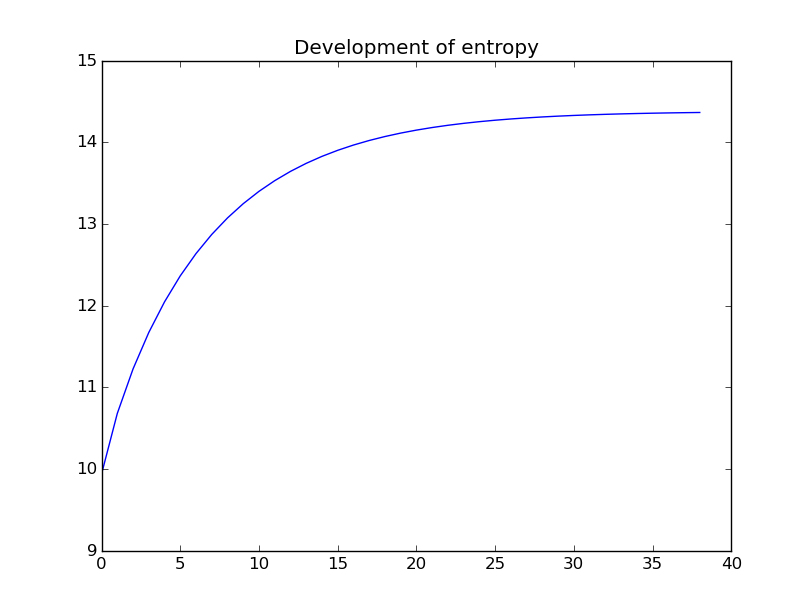
\includegraphics[width = \textwidth]{q6.png}
\end{figure}


\end{document}